\section{Iterative Calibration and MNL Re-Ranking}

\subsection{Calibration Ceiling}

A natural next step is to feed estimated parameters back into OTP's cost
function and iterate. Increasing walkReluctance from 1.0 to 5.0 and
transferCostSeconds from 120 to 300 proved counterproductive: the Exact Match
rate collapsed from 28.66\% to 14.0\%, because transit networks are
fundamentally discrete---a modest parameter shift can cause entirely different
routes to become Pareto-optimal. Holding the choice set fixed and optimizing
$\theta$ solely to improve ranking yields at most +1.02\%p (pooled MSA) or
+0.95\%p (probabilistic RSM, R\textsuperscript{2} = 0.98). In both cases, all
parameters converge to boundary values, and decomposition shows improvement is
driven almost entirely by MNL re-ranking of generated alternatives, not by the
router's own ranking improving. This establishes a structural ceiling of
approximately +1\%p for $\theta$-based calibration.

\subsection{MNL Re-Ranking: Core Contribution}

Rather than tuning the router's cost function, we re-rank OTP's existing
alternatives using estimated utility---no re-routing required:
\[
\mathrm{Rank}_{\mathrm{MNL}} = \arg\max_j V_j = \arg\max_j \boldsymbol{\beta}'\mathbf{x}_j
\]

\begin{table}[htbp]
\centering
\tablefont
\begin{tabular}{|l|c|c|r|}
\hline
\headrow
\textbf{Ranking Method} & \textbf{Exact Match} & \textbf{sim\_total} & \textbf{N} \\
\hline
OTP 1st Rank (gen.\ cost min)  & 20.34\%  & 0.5372 & 1,320,030 \\
\hline
MNL 1st Rank (V max)           & 22.23\%  & 0.5713 & 1,320,030 \\
\hline
Best Match (theoretical max)   & 28.66\%  & 0.6260 & 1,320,030 \\
\hline
MNL $-$ OTP Improvement        & +1.89\%p & +0.034 & ---       \\
\hline
\end{tabular}
\caption{MNL Re-Ranking vs.\ OTP Ranking (Full Dataset, N = 1,320,030)}
\end{table}

The gain is +1.89 percentage points on Exact Match---roughly double the
calibration ceiling---at a fraction of the cost (17 minutes of scoring vs.\
hours of iterative OTP execution). In 75.4\% of chains the two rankings agree;
among the 24.6\% (325,154 chains) where they diverge, MNL achieves Exact Match
10.4 times more often than OTP (27,608 vs.\ 2,663 chains) and outperforms on
sim\_total in 73.1\% of disagreements (win ratio 2.7:1).

\begin{figure}[htbp]
\centering
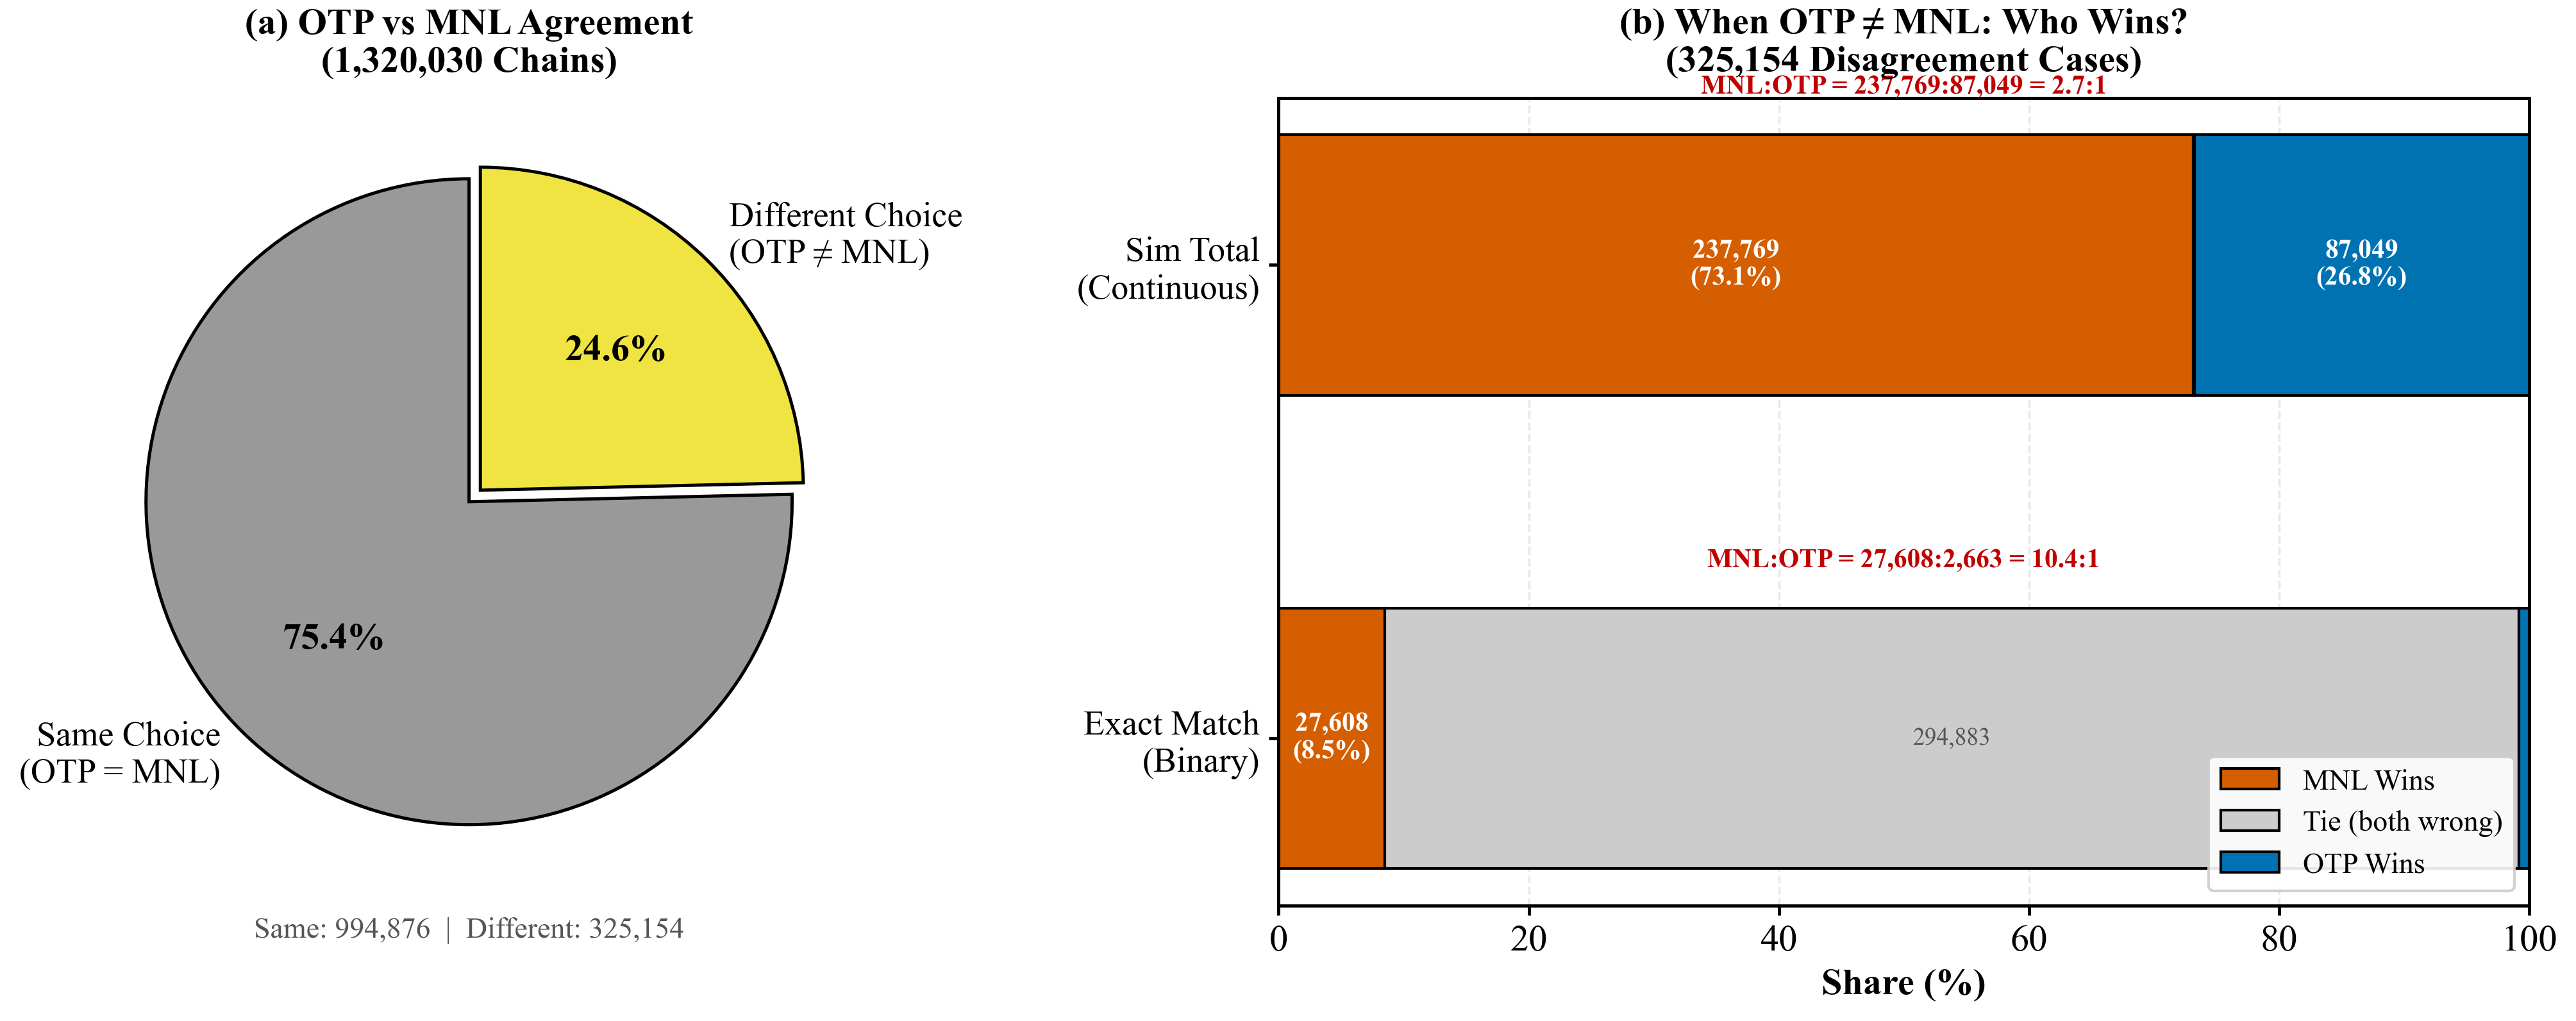
\includegraphics[width=0.98\textwidth]{figures/figure4_otp_mnl_disagreement.png}
\caption{OTP vs.\ MNL Disagreement: Win Ratios by Evaluation Metric}
\end{figure}

\subsubsection{Improvement Grows with Choice Set Richness}

\begin{table}[htbp]
\centering
\tablefont
\begin{tabular}{|c|r|c|c|c|}
\hline
\headrow
\textbf{Alternatives} & \textbf{Chains} & \textbf{OTP Exact} & \textbf{MNL Exact} & $\boldsymbol{\Delta}$ \\
\hline
1    & 345,967 (26.2\%) & 32.92\% & 32.92\% & +0.00\%p \\
\hline
2    & 170,755 (12.9\%) & 23.81\% & 25.33\% & +1.52\%p \\
\hline
3--4 & 332,660 (25.2\%) & 19.10\% & 21.33\% & +2.23\%p \\
\hline
5+   & 470,648 (35.7\%) & 10.72\% & 13.90\% & +3.17\%p \\
\hline
\end{tabular}
\caption{Re-Ranking Improvement by Number of Alternatives}
\end{table}

\begin{figure}[htbp]
\centering
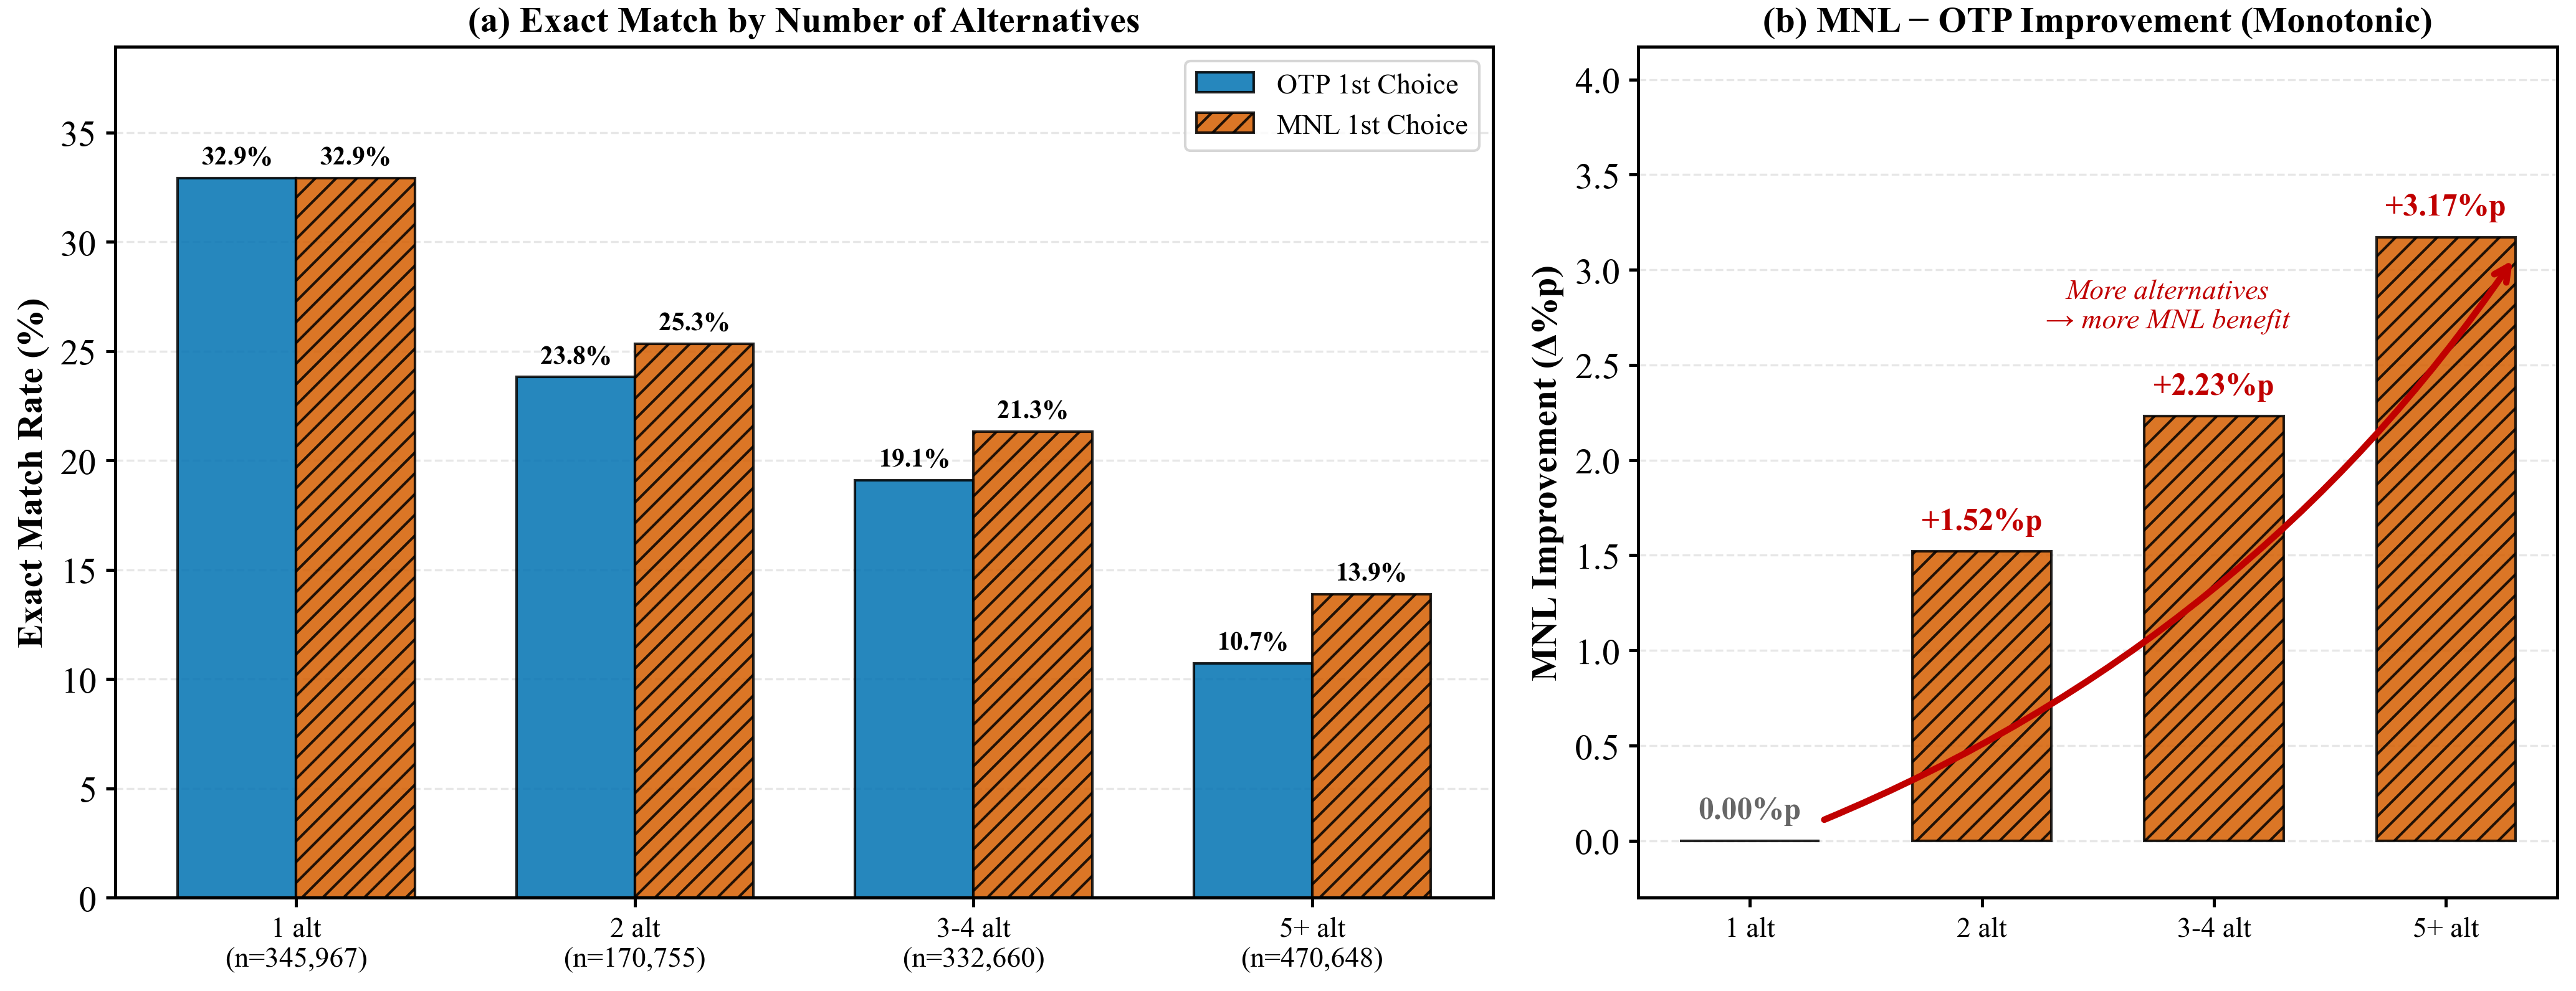
\includegraphics[width=0.98\textwidth]{figures/figure5_reranking_by_alternatives.png}
\caption{MNL Re-Ranking Improvement by Number of Available Alternatives}
\end{figure}

The improvement grows monotonically with choice set size: from zero where
only one alternative exists to +3.17\%p with five or more alternatives,
delivering its greatest value precisely where routing is most complex.

\subsubsection{What MNL-Selected Routes Look Like}

\begin{table}[htbp]
\centering
\tablefont
\begin{tabular}{|l|c|c|c|}
\hline
\headrow
\textbf{Attribute} & \textbf{OTP 1st Rank} & \textbf{MNL 1st Rank} & \textbf{Difference} \\
\hline
In-vehicle time (min) & 18.8   & 19.9   & +1.1 (+5.9\%)    \\
\hline
Walking time (min)    & 3.2    & 2.6    & $-0.6$ ($-18$\%) \\
\hline
Transfers (count)     & 0.50   & 0.40   & $-0.10$ ($-20$\%) \\
\hline
Subway ratio          & 61.5\% & 63.5\% & +2.0\%p          \\
\hline
\end{tabular}
\caption{Route Characteristics: OTP vs.\ MNL First-Ranked Routes}
\end{table}

Relative to OTP's top pick, MNL favors routes with 18\% less walking, 20\%
fewer transfers, and 2 percentage points more subway usage, at the cost of
5.9\% longer ride times. Given a walking weight of 22.7$\times$, the observed
trade-off is overwhelmingly favorable from the traveler's perspective. OTP's
default walkReluctance of 1.0 understates the true perceived burden by more
than an order of magnitude, which is the fundamental reason its rankings
diverge from observed behavior.
